% Thesis appendix item: clean_r2_vs_robustness
% Seeded on 2026-09-27 from qsar_qm_models/supplementary/items/clean_r2_vs_robustness.tex by thesis_appendix/seed_from_paper.py.
% From here on this copy is edited independently of the paper. Rules: thesis_appendix/README.md.
% The lines below, down to the first blank line, are the PAPER copy's header, kept for
% provenance. They describe the paper file, not this one: in particular a GENERATED
% notice there does not apply here, and this copy may be edited by hand.
% Supplementary item: clean_r2_vs_robustness
% Split out of additional_files.tex on 2026-09-27, where it was Additional file 7 (Baseline R^2 vs NDS scatter (was Supp Figure S2)).
% Content unchanged apart from: the heading line removed (the build writes it), the old
% 'Table S*/Figure S*' caption prefix replaced by \SuppFile{}, and the label renamed to supp:clean_r2_vs_robustness.
% Rules: supplementary/README.md.

\begin{figure}[H]
\centering
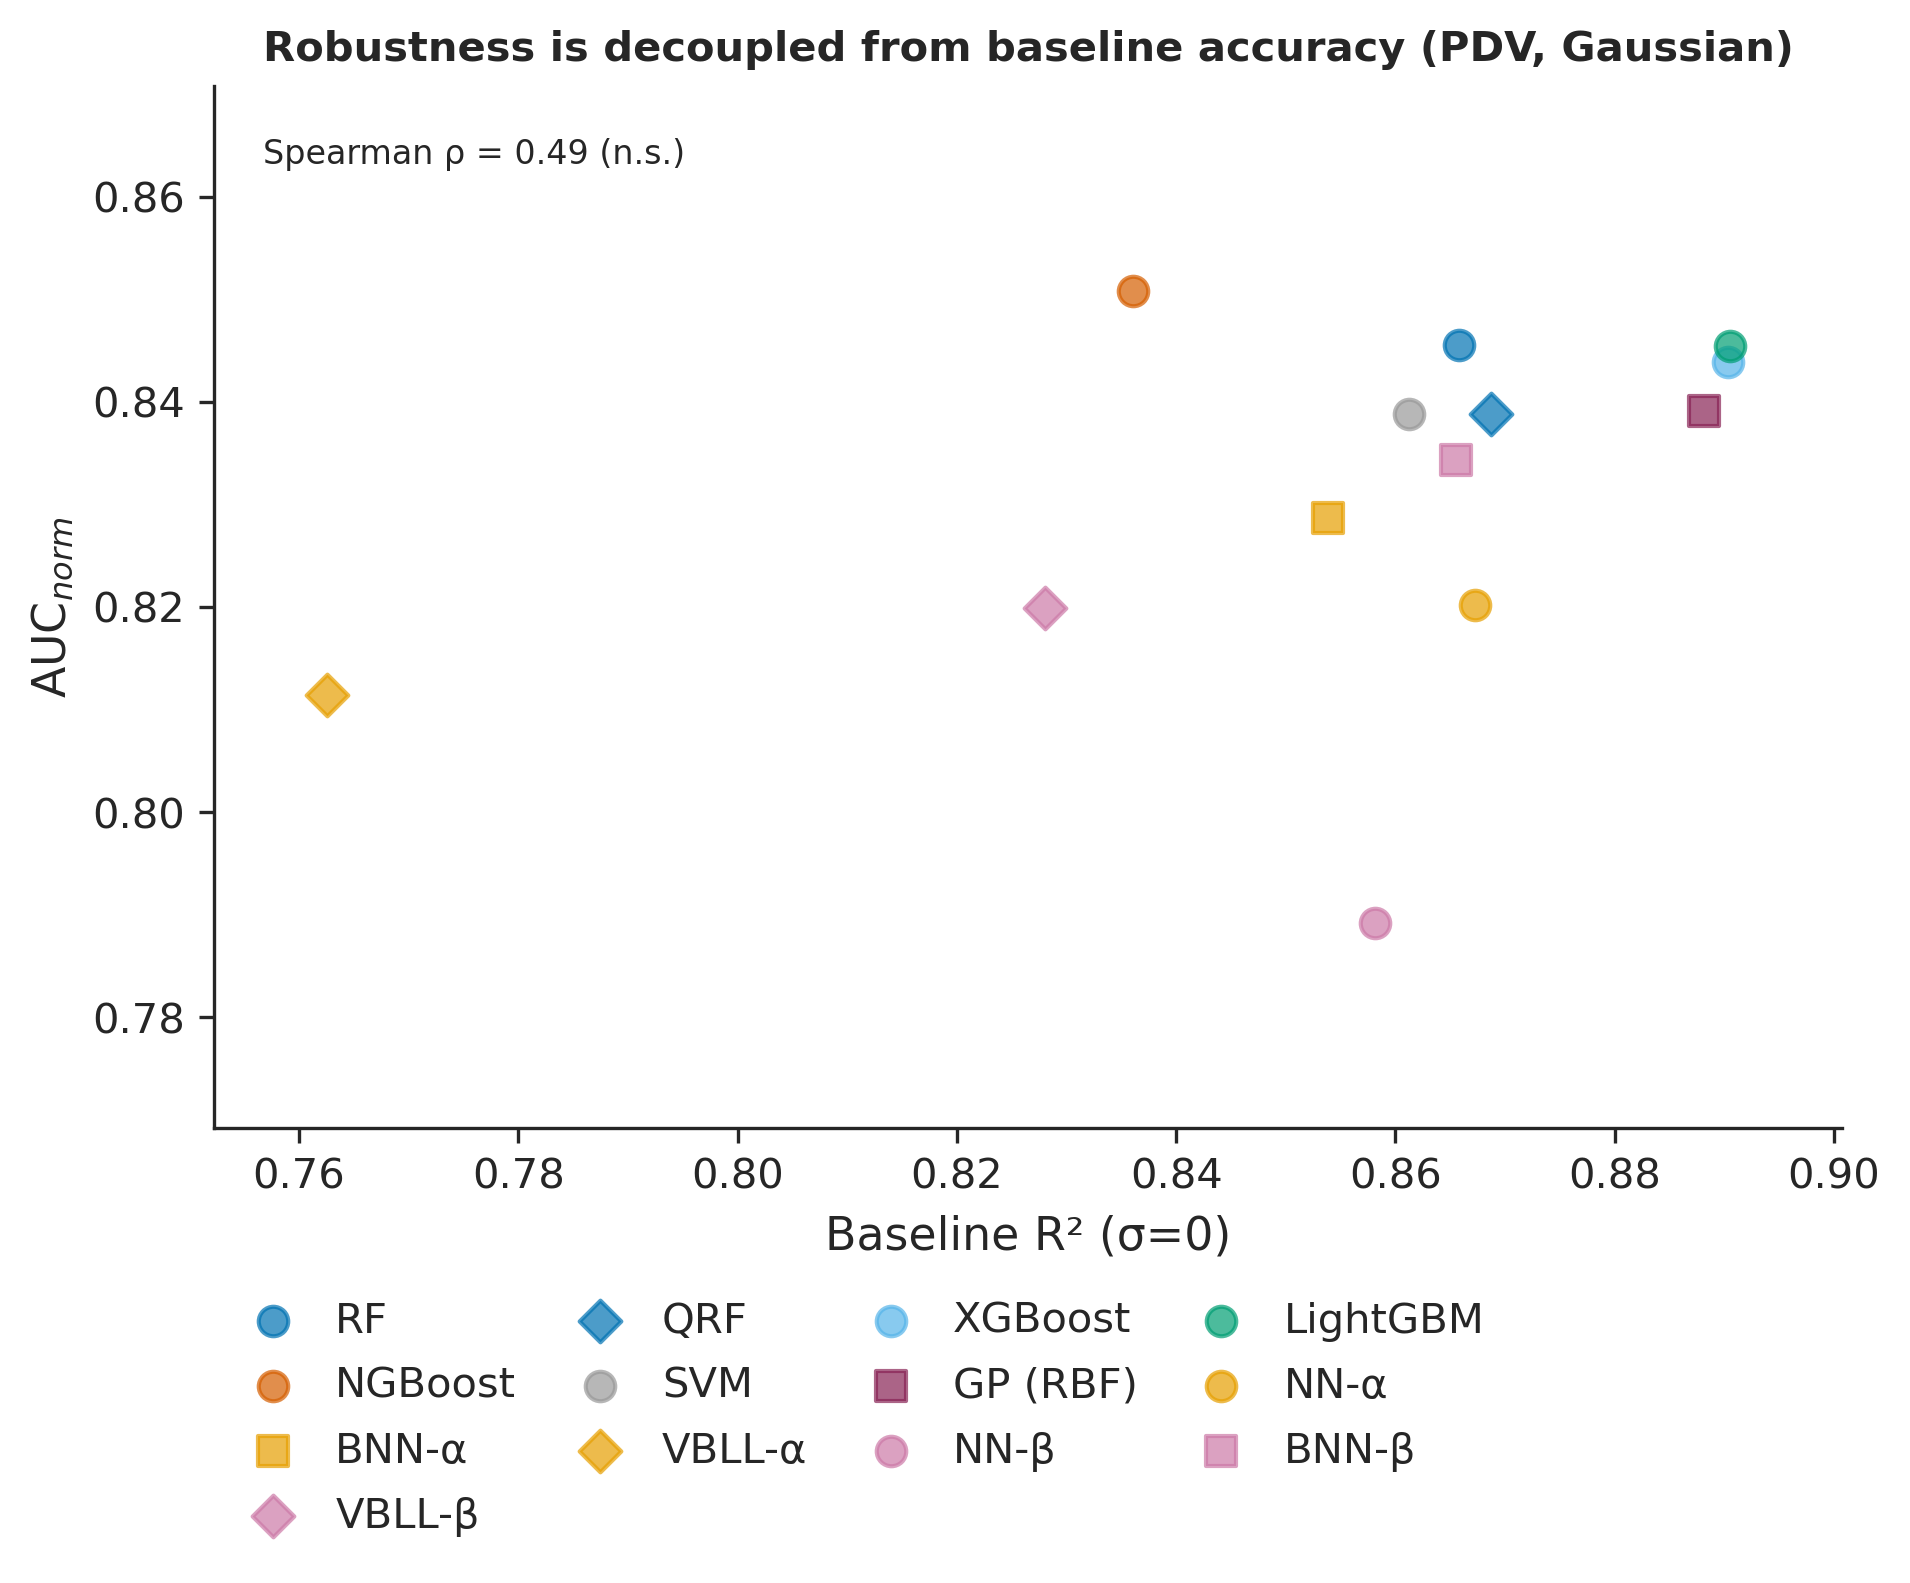
\includegraphics[width=\textwidth]{fig3_ranking_consistency.png}
\caption{\textbf{Baseline R$^2$ versus noise degradation slope (NDS) scatter for all models on the physicochemical descriptor vector (PDV) representation under Gaussian noise, on the QM9 HOMO--LUMO gap.}
Lower (more negative) NDS indicates faster performance loss under noise.}
\label{app:noise:clean_r2_vs_robustness}
\end{figure}
